La parte finale dell’elaborato consiste nell’utilizzare un modello già trainato per fargli produrre delle previsioni a fronte dell’inserimento di nuove immagini. Si sceglie quindi il modello dal quale si vogliono ottenere le previsioni, per far ciò basta copiare il file con estensione \texttt{.model}, corrispondente al modello scelto, nella cartella \texttt{PREDICTION}. Successivamente si inseriscono le immagini su cui si vuole avere un riscontro nella sottocartella di \texttt{PREDICTION}, \texttt{DATA\_TO\_PREDICT}. Infine si lancia lo script \texttt{predict.py}, che dopo un primo controllo sull’esistenza delle immagini e del modello nella cartella designata, invoca la funzione \texttt{make\_predictions} che al suo interno richiama la funzione \texttt{create\_data} di \texttt{preprocess.py}, in questo modo si fanno passare le nuove immagini attraverso tutte le diverse elaborazioni precedentemente descritte: filtri, threshold, Hough, segmentation e cropping. Grazie a questo passaggio si estraggono i segmenti di interesse dalle nuove immagini.

L’ultima operazione da effettuare prima di poter chiedere al modello di effettuare le previsioni è quella di resize dei nuovi segmenti. Infatti i segmenti prodotti da \texttt{create\_data} sotto generalmente di dimensione diversa, risulta quindi necessario ridimensionarli tutti alla stessa dimensione; tuttavia non li si può ridimensionare alla shape media come in precedenza, bisogna infatti ridimensionarli alla dimensione che il modello si aspetta di ricevere, in quanto il modello è stato addestrato per operare con immagini in input con quella particolare shape. La dimensione delle immagini in input richiesta dal modello è ottenibile accedendo all’attributo \texttt{input\_shape} dell’oggetto che rappresenta il modello stesso, successivamente si richiama la funzione \texttt{resize} di NumPy per ridimensionare i segmenti. 

A questo punto si può chiedere al modello di effettuare le previsioni, si richiama quindi la funzione \texttt{predict} sull’oggetto rappresentante il modello passandogli come parametro il vettore che contiene i segmenti ridimensionati. La funzione restituisce un array dove ogni elemento rappresenta il risultato della previsione per ogni immagine, se la previsione è 0 significa che la rete ha ritenuto il segmento come non problematico, mentre nel caso contrario ci sarà un 1 come previsione e quindi il segmento è stato reputato problematico. La funzione termina stampando sullo standard output il risultato della previsione associato al nome dell’immagine.

\begin{figure}[h]
  \centering
  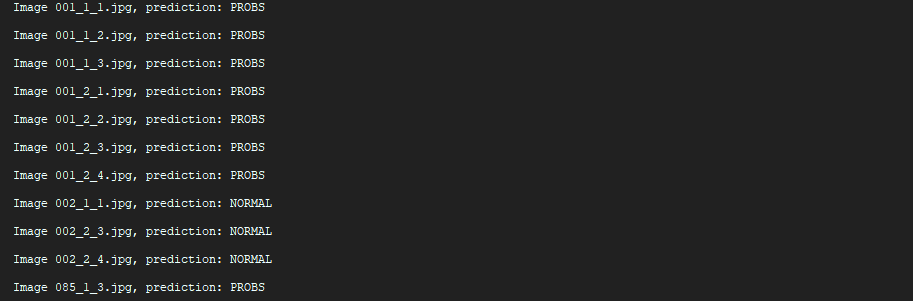
\includegraphics[width=1.0\textwidth]{predictions.png}
  \caption{Esempio di output ottenuto lanciando \texttt{predict.py}}
\end{figure}
